\documentclass[border=1mm, convert]{standalone}
%\documentclass{article}
\usepackage{tikz}
\usetikzlibrary{arrows}
\usetikzlibrary{calc}

\begin{document}

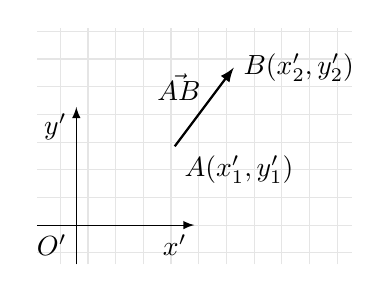
\begin{tikzpicture}[line/.style={>=latex}] 
\coordinate (O) at (-.5, 0);
\coordinate (A) at (.75, 1);
\coordinate (B) at (1.5, 2);

%\draw[step=10pt, color=white] (-.5, -.5) grid (2.5, 2.5);
\draw[step=10pt, color=black!10] (-1, -.5) grid (3, 2.5);
\draw[->, line] (-1, 0) -- node [below, very near end] {$x'$} (1, 0);
\draw[->, line] (-.5, -.5) -- node [left, very near end] {$y'$} (-.5, 1.5);

\node at (O) [below left] {$O'$};
\node at (A) [below right] {$A (x'_1,y'_1)$};
\node at (B) [below, right] {$B (x'_2,y'_2)$};
\draw[->, line, thick] (A) -- node [left=3pt, near end]    {$\vec{AB}$} (B);

\end{tikzpicture}
\end{document}